\documentclass[11pt,a4paper]{article}
\usepackage[spanish,es-nodecimaldot]{babel}	% Utilizar español
\usepackage[utf8]{inputenc}					% Caracteres UTF-8
\usepackage{graphicx}						% Imagenes
\usepackage[hidelinks]{hyperref}			% Poner enlaces sin marcarlos en rojo
\usepackage{fancyhdr}						% Modificar encabezados y pies de pagina
\usepackage{float}							% Insertar figuras
\usepackage[textwidth=395pt]{geometry}		% Anchura de la pagina
\usepackage[nottoc]{tocbibind}				% Referencias (no incluir num pagina indice en Indice)
\usepackage{enumitem}						% Permitir enumerate con distintos simbolos
\usepackage[T1]{fontenc}					% Usar textsc en sections
\usepackage{amsmath}						% Símbolos matemáticos
\usepackage{algorithm}						% Environtment algorithm
\usepackage[noend]{algpseudocode}			% Pseudocodigo
\usepackage{listings}

\algnewcommand\algorithmicforeach{\textbf{for each}}
\algdef{S}[FOR]{ForEach}[1]{\algorithmicforeach\ #1\ \algorithmicdo}

\algrenewcommand\algorithmicreturn{\textbf{return}}


\lstset{
	language=bash
}

% Comando para poner el nombre de la asignatura
\newcommand{\asignatura}{Metaheurísticas}
\newcommand{\autor}{Vladislav Nikolov Vasilev}

% Configuracion de encabezados y pies de pagina
\pagestyle{fancy}
\lhead{\autor{}}
\rhead{\asignatura{}}
\lfoot{Grado en Ingeniería Informática}
\cfoot{}
\rfoot{\thepage}
\renewcommand{\headrulewidth}{0.4pt}		% Linea cabeza de pagina
\renewcommand{\footrulewidth}{0.4pt}		% Linea pie de pagina

\begin{document}
\pagenumbering{gobble}

% Pagina de titulo
\begin{titlepage}

\begin{minipage}{\textwidth}

\centering


\includegraphics[scale=0.3]{img/ugr.png}\\

\textsc{\Large \asignatura{}\\[0.2cm]}
\textsc{GRADO EN INGENIERÍA INFORMÁTICA}\\[0.3cm]

\noindent\rule[-1ex]{\textwidth}{1pt}\\[1.5ex]
\textsc{{\Huge PRÁCTICA 2\\[1pt]}}
\textsc{{\Large \\Técnicas de Búsqueda basadas en Poblaciones para el Problema del Aprendizaje de Pesos en Características}}
\noindent\rule[-1ex]{\textwidth}{2pt}\\[1ex]

\end{minipage}

\vspace{0.18cm}

\begin{minipage}{\textwidth}

\centering

\textbf{Autor}\\ {\autor{}}\\[1ex]
\textbf{NIE}\\ {X8743846M}\\[1ex]
\textbf{E-Mail}\\ {vladis890@gmail.com}\\[1ex]
\textbf{Grupo de prácticas}\\ {MH3 Jueves 17:30-19:30}\\[1ex]
\textbf{Rama}\\ {Computación y Sistemas Inteligentes}\\[1ex]
\vspace{0.2cm}


\includegraphics[scale=0.3]{img/etsiit.jpeg}

\vspace{0.3cm}
\textsc{Escuela Técnica Superior de Ingenierías Informática y de Telecomunicación}\\
\vspace{1cm}
\textsc{Curso 2018-2019}
\end{minipage}
\end{titlepage}

\pagenumbering{arabic}
\tableofcontents
\thispagestyle{empty}				% No usar estilo en la pagina de indice

\newpage

\setlength{\parskip}{1em}

\section{Descripción del problema}

El problema que se aborda en esta práctica es el Aprendizaje de Pesos en Características (APC). Es un problema típico de
\textit{machine learning} en el cuál se pretende optimizar el rendimiento de un clasificador basado en vecinos más cercanos.
Esto se consigue mediante la ponderación de las características de entrada con un vector de pesos $W$, el cuál utiliza
codificación real (cada $w_i \in W$ es un número real), con el objetivo de modificar sus valores a la hora de calcular la
distancia. Cada vector $W$ se expresa como $W = \lbrace w_1, w_2, \dots , w_n \rbrace$, siendo $n$ el número de dimensiones
del vector de características, y cumpliéndose además que $\forall w_i \in W, \; w_i \in [0, 1]$.\par

El clasificador considerado para este problema es el 1-NN (genéricamente, un clasificador $k$-NN, con $k$ vecinos, siendo
en este caso $k = 1$), es decir, aquél que clasifica un elemento según su primer vecino más cercano utilizando alguna medida
de distancia (en este caso, utilizando la distancia Euclídea). Cabe destacar que no en todos los casos se usará el clasificador
1-NN ya que se pueden dar casos en los que el vecino más cercano de un elemento sea él mismo. Por ese motivo, en algunas
técnicas/algoritmos se usará un 1-NN con el criterio de \textit{leave-one-out}, es decir, que se busca el vecino más cercano
pero excluyéndose a él mismo.\par

El objetivo propuesto es aprender el vector de pesos $W$
mediante una serie de algoritmos, de tal forma que al optimizar el clasificador se mejore tanto la precisión de éste como su
complejidad, es decir, que se considere un menor número de características. Estos dos parámetros, a los que llamaremos $tasa\_
clas$ y $tasa\_red$, respectivamente, se pueden expresar de la siguiente forma:

\[tasa\_clas = 100 \cdot \frac{nº \; instancias \; bien \; clasificadas \; en \; T}{nº \; instancias \; en \; T}\]
\[tasa\_red = 100 \cdot \frac{nº \; valores \; w_i < 0.2}{nº \; caracteristicas}\]

\noindent siendo $T$ el tamaño del conjunto de datos sobre que el que se evalúa el clasificador.\par

Por tanto, al combinarlos en una única función a la que llamaremos $F(W)$, la cuál será nuestra función objetivo a optimizar
(maximizar), tenemos que:

\[F(W) = \alpha \cdot tasa\_clas(W) + (1 - \alpha) \cdot tasa\_red(W)\] 

\noindent siendo $\alpha$ la importancia que se le asigna a la tasa de clasificación y a la de reducción, cumpliendo que
$\alpha \in [0, 1]$. En este caso, se utiliza un $\alpha = 0.5$ para dar la misma importancia a ambos, con lo cuál se pretende
que se reduzcan al máximo el número de características conservando una $tasa\_clas$ alta.

\section{Descripción de los algoritmos}

\subsection{Consideraciones previas}

Antes de empezar con la descripción formal de los algoritmos implementados, vamos a describir algunos aspectos
comunes, como por ejemplo cómo se representan e inicializan las soluciones; cómo se representan la población, los padres y las
elecciones para mutar los cromosomas; cómo se realiza el torneo binario, la mutación y los distintos cruces, y algunas funciones
utilizadas en muchas partes del código, como por ejemplo la función objetivo o la forma de evaluar a la población. Cabe destacar
que muchos de los pseudocódigos que aparecen a continuación no se han implementado exactamente igual o no aparecen en el
código, ya que o bien son operaciones que se han vectorizado o bien ya hay funciones que hacen eso.

Primero vamos a ver como se representa la población, los padres y una elección de mutación. Una población no es más que un
vector de vectores, o lo que es lo mismo, una matriz de tamaño $N \times M$, donde $N$ es el número de cromosomas (soluciones)
y $M$ es el número de genes (número de características). Por tanto, ahora tenemos un conjunto de vectores de pesos, lo que
viene a significar que tenemos múltiples $W$. Esta población está ordenada en todo momento por el valor \textit{fitness}
de cada cromosoma para facilitar las operaciones posteriores. Un padre $p$ no es más que un índice de un cromosoma de la
población, con la restricción de que $p \in [0, N)$. Una mutación viene dada por dos valores $c, g$, donde $c$ es el cromosoma
a mutar y $g$ el gen a mutar. Estos dos valores están sujetos a que $c \in [0, N)$ y a que $g \in [0, M)$.

Como cada fila de la matriz es un vector de pesos $W$, se tiene que cumplir que $\forall w_i \in W, \; w_i \in [0, 1]$. Por
tanto, para evitar que las soluciones se salgan de este intervalo, se ha implementado una función que se encarga de normalizar
los valores de $W$ en el rango. La función se ha usado tanto en los algoritmos meméticos como en los genéticos a
la hora de realizar un cruce o una mutación, para que los valores de los cromosomas siguiesen siendo válidos. La
implementación de esta función es la siguiente:

\begin{algorithm}[H]
\caption{Función que normaliza un vector de pesos $W$}
\begin{algorithmic}[1]
\Function{NormalizarW}{$W$}
\ForEach{$w_i \in W$}
	\If{$w_i < 0$}
		\State $w_i \gets 0$
	\ElsIf{$w_1 > 1$}
		\State $w_i \gets 1$
	\EndIf
\EndFor
\State \Return{$W$}
\EndFunction
\end{algorithmic}
\end{algorithm}

Para generar las soluciones iniciales se ha utilizado una función que recibe como parámetros el número de genes y el número de
cromosomas, y crea una nueva matriz que representa la población, inicializándola con valores aleatorios generados
mediante una distribución uniforme en el rango $[0, 1]$. Su pseudocódigo se puede ver a continuación:

\begin{algorithm}[H]
\caption{Función que genera una población inicial}
\begin{algorithmic}[1]
\Function{GenerarPoblacionInicial}{$numCrom$, $numGenes$}
\State $poblacion \gets $ NuevaMatrizVacia($numCrom$, $numGenes$)
	\For{$i \gets 0$ \textbf{to} $numCrom - 1$}
		\For{$j \gets 0$ \textbf{to} $numGenes- 1$}
			\State $poblacion[i][j] \gets $ ValorAleatorioUniformeRango0-1()
		\EndFor	
	\EndFor
\State \Return{$poblacion$}
\EndFunction
\end{algorithmic}
\end{algorithm}

Para seleccionar los padres o cromosomas que pasarán su material genético se ha utilizado una función que recibe los índices
de 2 cromosomas y la lista de valores \textit{fitness}, y devuelve el índice del cromosoma con mejor valor \textit{fitness}.
Se muestra su implementación a continuación:

\begin{algorithm}[H]
\caption{Función que realiza un torneo binario y elige el mejor padre}
\begin{algorithmic}[1]
\Function{TorneoBinario}{$listaFitness$, $indxCrom1$, $indxCrom2$}
\State $fitCrom1 \gets listaFitness[indxCrom1]$
\State $fitCrom2 \gets listaFitness[indxCrom2]$
\State $mejorPadre \gets indxCrom1$
\If{$ fitCrom1 < fitCrom2$}
	\State $mejorPadre \gets indxCrom2$
\EndIf
\State \Return{$mejorPadre$}
\EndFunction
\end{algorithmic}
\end{algorithm}

En cuanto a los cruces, para el cruce BLX-$\alpha$ se ha creado una función que recibe la población, los índices
de los padres y aplica el cruce, generando dos descendientes. En este caso se ha especificado que $\alpha = 0.3$.
Aquí se puede ver como funciona:

\begin{algorithm}[H]
\caption{Cruce BLX-$\alpha$ con $\alpha = 0.3$ (I)}
\begin{algorithmic}[1]
\Function{CruceBLXAlfa}{$poblacion$, $indPadre1$, $indPadre2$, $numGenes$, $\alpha$}
\State $padre1$, $padre2 \gets poblacion[indPadre1]$, $poblacion[indPadre2]$
\State $hijo1$, $hijo2$, $C_{min}$, $C_{max}$, $I \gets$ NuevoVectorVacio($numGenes$)
\For{$i \gets 0$ \textbf{to} $numGenes - 1$}
	\State $C_{min}[i] \gets$ Minimo($padre1[i]$, $padre2[i]$)
	\State $C_{max}[i] \gets$ Maximo($padre1[i]$, $padre2[i]$)
	\State $I[i] \gets C_{max}[i] - C_{min}[i]$)
\EndFor
\algstore{blx}
\end{algorithmic}
\end{algorithm}

\begin{algorithm}[H]
\caption{Cruce BLX-$\alpha$ con $\alpha = 0.3$ (II)}
\begin{algorithmic}[1]
\algrestore{blx}
\For{$i \gets 0$ \textbf{to} $numGenes - 1$}
	\State $hijo1[i] \gets$ ValorAleatorioUnifInter($C_{min}[i] - I[i] \cdot \alpha$, $C_{max}[i] + I[i] \cdot \alpha$)
	\State $hijo2[i] \gets$ ValorAleatorioUnifInter($C_{min}[i] - I[i] \cdot \alpha$, $C_{max}[i] + I[i] \cdot \alpha$)
\EndFor
\State NormalizarW($hijo1$), NormalizarW($hijo2$)
\State \Return{$hijo1$, $hijo2$}
\EndFunction
\end{algorithmic}
\end{algorithm}

Para el cruce aritmético (AC) se ha implementado una función que recibe la población y los índices de los padres, y genera
los descendientes haciendo la media aritmética, como se puede ver aquí:

\begin{algorithm}[H]
\caption{Función del cruce aritmético}
\begin{algorithmic}[1]
\Function{CruceAritmetico}{$poblacion$, $indPad1$, $indPad2$, $numGenes$}
\State $padre1$, $padre2 \gets poblacion[indPad1]$, $poblacion[indPad2]$
\State $hijo \gets$ NuevoVectorVacio($numGenes$)
\For{$i \gets 0$ \textbf{to} $numGenes - 1$}
	\State $hijo[i] \gets (padre1[i] + padre2[i])$ / 2
\EndFor
\State \Return{$hijo$}
\EndFunction
\end{algorithmic}
\end{algorithm}

Para la mutación se ha creado una función que recibe la población y los índices del cromosoma y gen a mutar, y añade a dicho
gen un valor generado por una distribución normal con $\mu = 0$ y $\sigma = 0.3$. Se puede ver a continuación:

\begin{algorithm}[H]
\caption{Función de mutación}
\begin{algorithmic}[1]
\Procedure{Mutacion}{$pob$, $indCrom$, $indGen$}
\State $pob[indCrom][indGen] \gets pob[indCrom][indGen] + $ ValorDistribNorm($\mu$, $\sigma$)
\State NormalizarW($pob[indCrom]$)
\EndProcedure
\end{algorithmic}
\end{algorithm}

Vamos a comentar ahora algunos detalles extra. Es importante saber como se calcula la distancia a un vecino, ya que esto juega
un factor muy importante a la hora de encontrar cuál es el vecino más cercano a un elemento (o el vecino más cercano por el
criterio \textit{leave-one-out}). En la implementación de la práctica se ha utilizado un KDTree, que es una estructura de datos
parecida a un árbol binario, solo que de $K$ dimensiones. Por dentro, esta estructura utiliza la distancia Euclídea (distancia
en línea recta entre dos elementos) para determinar cuál es el elemento más próximo a otro. No hace falta conocer como se
implementa esta estructura de datos, pero sí es importante conocer cómo se realiza el cálculo de la distancia Euclídea. En el
siguiente pseudocódigo se puede ver el cálculo:

\begin{algorithm}[H]
\caption{Cálculo de la distancia Euclídea entre dos puntos}
\begin{algorithmic}
\Function{DistanciaEuclidea}{$e_1, e_2$}
\State $distancia \gets \sqrt{\sum_{i=1}^{N} (e_1^i - e_2^i)^2}$
\State \Return{$distancia$}
\EndFunction
\end{algorithmic}
\end{algorithm}

También es importante ver cómo se mantiene la población ordenada. Para hacer esto, se ha creado una función que recibe la
lista de valores \textit{fitness} y la poblacion, obtiene los índices que dan el orden de forma ascendente de la lista
y con estos índices ordena la población y la lista de \textit{fitness}. Aquí se puede ver como funciona:

\begin{algorithm}
\caption{Función para ordenar la población según su valor \textit{fitness}}
\begin{algorithmic}[1]
\Function{OrdenarPoblacionPorFitness}{$fitness$ , $poblacion$}
\State $indicesOrden \gets $ ObtenerIndicesOrdenados($fitness$)
\State $fitnessOrdenado \gets$ NuevoVectorVacioMismaCapacidad($fitness$)
\State $poblacionOrdenada \gets$ NuevaMatrizVaciaMismaCapacidad($poblacion$)
\ForEach{$indice \in indicesOrden$}
	\State $fitnessOrdenado \gets fitness[indice]$
	\State $poblacionOrdenada \gets poblacion[indice]$
\EndFor
\State \Return{$fitnessOrdenado$, $poblacionOrdenada$}
\EndFunction
\end{algorithmic}
\end{algorithm}

Pasemos a ver ahora la función objetivo, $F(W)$, que es lo que se pretende optimizar. Para evaluar la función objetivo,
necesitamos calcular $tasa\_clas$ y $tasa\_red$. Para calcular lo primero, podemos seguir la idea detrás del siguiente
pseudocódigo:

\begin{algorithm}[H]
\caption{Cálculo de la tasa de clasificación}
\begin{algorithmic}[1]
\Function{CalculoTasaClas}{$etiq, etiqPred, N$}
\State $bienClasificados \gets 0$
\For{$i \gets 1$ \textbf{to} $N$}
	\If{$etiq_i = etiqPred_i$}
		\State $bienClasificados \gets bienCasificados + 1$
	\EndIf
\EndFor
\State $tasa\_clas \gets bienClasificados$ / $N$
\State \Return{$tasa\_clas$}
\EndFunction
\end{algorithmic}
\end{algorithm}

Para calcular $tasa\_red$, suponiendo que queremos saber el número de características por debajo de $0.2$ podemos seguir un
esquema como el siguiente:

\begin{algorithm}[H]
\caption{Cálculo de la tasa de reducción (I)}
\begin{algorithmic}[1]
\Function{CalculoTasaRed}{$W, N$}
\State $caracRed \gets 0$
\ForEach{$w_i \in W$}
\algstore{reduction}
\end{algorithmic}
\end{algorithm}

\begin{algorithm}[H]
\caption{Cálculo de la tasa de reducción (II)}
\begin{algorithmic}
\algrestore{reduction}
	\If{$w_i < 0.2$}
		\State $caracRed \gets caracRed + 1$
	\EndIf
\EndFor
\State $tasa\_red \gets caracRed$ / $N$
\State \Return{$tasa\_red$}
\EndFunction
\end{algorithmic}
\end{algorithm}

Y finalmente, para poder calcular la función a optimizar (nuestra función \textit{fitness} u objetivo), teniendo en cuenta que
usamos un $\alpha = 0.5$ para ponderar las dos tasas, y que anteriormente hemos calculado ambas tasas, podemos seguir el
siguiente esquema:

\begin{algorithm}[H]
\caption{Cálculo de la función objetivo o \textit{fitness}}
\begin{algorithmic}[1]
\Function{CalculoFuncionFitness}{$tasa\_clas, tasa\_red, \alpha$}
\State $fitness \gets \alpha \cdot tasa\_clas + (1 - \alpha) \cdot tasa\_red$
\State \Return{$fitness$}
\EndFunction
\end{algorithmic}
\end{algorithm}

Para acabar, y antes de pasar a ver la implementación de los algoritmos, veamos otra funcionalidad que se usa en todos los
algoritmos, que es la forma en la que se evalúa la función objetivo. Para eso, se usa una función que permite evaluar a toda la
nueva población, la cuál a su vez llama a una función que evalúa cada elemento de la población. Veamos su funcionamiento,
empezando por la función más específica (la cuál solo evalúa un vector de pesos $W$) hasta la más genérica:

\begin{algorithm}[H]
\caption{Función para evaluar un vector de pesos $W$}
\begin{algorithmic}[1]
\Function{Evaluar}{$datos$, $etiquetas$, $W$}
\State $datosPesos \gets$ aplicar $w_i \in W$ sobre los $x_i \in datos$ donde $w_i > 0.2$
\State $arbolKD \gets$ KDTree($datosPesos$)
\State $vecinos \gets arbolKD$.ObtenerVecinosMasCercanoL1O($datosPesos$)
\State $pred \gets etiquetas[vecinos]$
\State $tasa\_clas \gets$ CalcularTasaClas($etiquetas$, $pred$, num. etiquetas)
\State $tasa\_red \gets$ CalcularTasaRed($W$, num. caracteristicas)
\State $fitness \gets$ CalculoFuncionFitness($tasa\_clas$, $tasa\_red$)
\State \Return{$fitness$}
\EndFunction
\end{algorithmic}
\end{algorithm}

\begin{algorithm}[H]
\caption{Función para evaluar una población}
\begin{algorithmic}[1]
\Function{EvaluarPoblacion}{$datos$, $etiquetas$, $poblacion$}
\State $listaFitness \gets $ NuevoVector()
\ForEach{$W \in poblacion$}
	\State $listaFitness$.Añadir(Evaluar($datos$, $etiquetas$, $W$))
\EndFor
\State \Return{$listaFitness$}
\EndFunction
\end{algorithmic}
\end{algorithm}

\subsection{Algoritmos de comparación}

\subsection{Algoritmos de búsqueda basados en poblaciones}

\newpage

\section{Desarrollo de la práctica}

La práctica se ha implementado en \textbf{Python3} y ha sido probada en la versión 3.7.1. Por tanto, se recomienda
encarecidamente utilizar un intérprete de Python3 al ejecutar el código y no uno de la versión 2.X, debio a problemas
de compatibilidad con ciertas funciones del lenguaje. Se ha probado el código sobre Linux Mint 19 y al estar basado en
Ubuntu 18 no debería haber problemas de compatibilidad con otros sistemas, además de que Python es un lenguaje muy portable.
No se ha probado en el entorno \textbf{conda}, pero si se consiguen instalar los módulos necesarios, no debería haber
problemas.

A la hora de implementar el software, se han utilizado tanto módulos ya incluidos en Python, como el módulo \textbf{time}
para la medición de tiempos, como módulos científicos y para \textit{machine learning}, como por ejemplo \textbf{numpy} y
\textbf{sklearn}. Este último se ha utlizado para poder dividir los datos para el \textbf{5 Fold Cross Validation}
y para obtener un clasificador KNN que poder utilizar para poder probar los resultados obtenidos por cada uno de los
algoritmos. Para la visualización de datos se ha utilizado \textbf{pandas}, ya que permite conseguir una visualización rápida
de estos gracias a los DataFrames.

Adicionalmente, la estructura de \textbf{KDTree} utilizada ha sido sacada de un módulo externo llamado
\textbf{pykdtree}\cite{pykdtree}. Este módulo está implementado en \textbf{Cython} y \textbf{C} y también utiliza
\textbf{OMP}, con lo cuál su rendimiento va a ser muy superior a otras implementaciones como por ejemplo el \textbf{cKDTree}
de \textbf{scipy}\footnote{De hecho, pykdtree está basado en cKDTree y libANN, cogiendo lo
mejor de cada implementación y paralelizando el código con OMP para conseguir unos rendimientos muy superiores a ambos,
tanto a la hora de crear el árbol como para hacer consultas.}. En cuanto a su uso, las funciones y la forma de construirlo
son las mismas que las de cKDTree, con lo cuál se puede consultar su documentación\cite{ckdtree} para obtener más información
sobre su uso.

Siendo ahora más concretos en cuanto a la implementación, se ha creado un módulo que contiene tanto código reutilizado de la
práctica anterior (creación de particiones, búsqueda local, función de normalización de los datos y funciones objetivo y de
evaluación de los datos) como código referente a esta práctica (es decir, la implementación de los algoritmos genéticos y
meméticos). Se ha implementado un algoritmo por cada estrategia del genético (un algoritmo para el AGG y uno para el AGE),
dando la posibilidad de elegir el operador de cruce a utilizar en cada caso, y una función para el algoritmo memético, que de
nuevo, ofrece la posibilidad de escoger la estrategia a utilizar. Además, se han implementado una serie de funciones a las
que se ha llamado clasificadores, que se encargan de recorrer las particiones creadas, de ejecutar los respectivos algoritmos
pasándoles los datos, entrenar luego un clasificador 1-NN con los pesos calculados y predecir las clases, además de recopilar
información estadística para mostrarla luego por pantalla. 

Se han utilizado dos semillas aleatorias las cuáles están fijas en el código: una para dividir los datos, y otra para los
algoritmos implementados, que se fija al justo antes de llamar a la función que le pasa los datos al algoritmo que se vaya a
ejecutar. Los ficheros ARFF proporcionados se han convertido al formato CSV con un script propio, con el objetivo de facilitar
la lectura de los datos. Estos archivos también se proporcionan junto con el código fuente implementado.

\newpage

\section{Manual de usuario}

Para poder ejecutar el programa, se necesita un intérprete de \textbf{Python3}, como se ha mencionado anteriormente. Además,
para poder satisfacer las dependencias se necesita el gestor de paquetes \textbf{pip} (preferiblemente \textbf{pip3}).

Se recomienda instalar las dependencias, las cuáles vienen en el archivo \textbf{requirements.txt}, ya que sin ellas, el
programa no podrá funcionar. Se recomienda utilizar el script de bash incluido para realizar la instalación, ya que se
encarga de instalarlo en un entorno virtual para no causar problemas de versiones con paquetes que ya se tengan instaladas en
el equipo o para no instalar paquetes no deseados. Una vez instalados\footnote{Si se produce algún error durante la
instalación de los paquetes, puede ser debido a pykdtree, ya que al necesitar un compilador que soporte OMP puede fallar en
los sistemas OSX. Para evitar estos problemas, el programa puede utilizar un cKDTree de scipy en caso de que a la hora de
importar pykdtree se produzca un error, suponiendo a cambio una penalización en el tiempo de ejecución.}, para poder utilizar
el entorno creado se debe ejecutar el siguiente comando:

\begin{lstlisting}
	$ source ./env/bin/activate
\end{lstlisting}

Para desactivar el entorno virtual, simplemente basta con ejecutar:

\begin{lstlisting}
	(env) $ deactivate
\end{lstlisting}

Para ejecutar el programa basta con ejecutar el siguiente comando:

\begin{lstlisting}
	$ python3 practica2.py [archivo] [algoritmo]
\end{lstlisting}

Los argumentos \textbf{archivo} y \textbf{algoritmo} son obligatorios, y sin ellos el programa lanzará una excepción. En
cuanto a sus posibles valores:

\begin{itemize}[label=\textbullet]
	\item \textbf{archivo} puede ser: \textbf{colposcopy}, \textbf{ionosphere} o \textbf{texture}.
	\item \textbf{algoritmo} puede ser:
	\begin{itemize}[label=$\ast$]
		\item Para AG: \textbf{genetics-generational-blx}, \textbf{genetics-generational-ac},\\
		\textbf{genetics-stationary-blx} o \textbf{genetics-stationary-ac}.
		\item Para AM: \textbf{memetics-all}, \textbf{memetics-best} o \textbf{memetics-rand}.
	\end{itemize}
\end{itemize}

A continuación, para ilustrar mejor lo explicado hasta el momento, se ofrece una captura de un ejemplo de ejecución del
programa. En la imagen se puede ver la siguiente información:

\begin{itemize}[label=\textbullet]
	\item Se muestra primero el conjunto de datos sobre el que se va a ejecutar, el clasificador que se va a ejecutar,
	las opciones que se le pasan a ese clasificador (que determinaran qué algoritmo utilizar) y el tiempo total.
	\item Se puede ver una tabla en la que aparecen los datos referentes a cada partición (tasa de clasificación, tasa de
	reducción, agrupación y tiempo).
	\item Se muestran valores estadísticos para cada variable (valores máximo, mínimo, medio, mediana y desviación típica).
\end{itemize}


\begin{figure}[H]
\centering
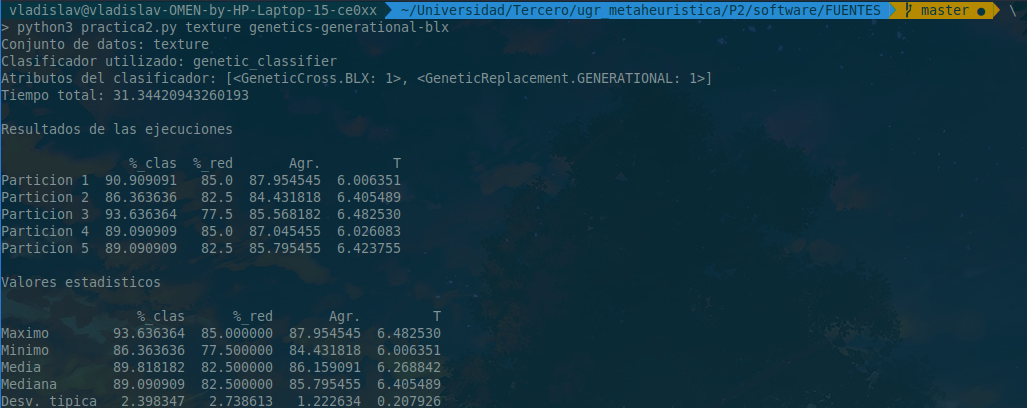
\includegraphics[scale=0.4]{img/out_example.png}
\caption{Ejemplo de salida de la ejecución con los datos \textbf{texture} y el \textbf{AGG}
con operador de cruce BLX-$\alpha$.}
\end{figure}

\newpage

\section{Análisis de resultados y experimentación}

\subsection{Descripción de los casos del problema}

Para analizar el rendimiento de los algoritmos, se han realizado pruebas sobre 3 conjuntos de datos:

\begin{itemize}[label=\textbullet]
	\item \textbf{Colposcopy}: Conjunto de datos de colposcopias adquirido y anotado por médicos profesionales del Hospital
	Universitario de Caracas. Las imágenes fueron tomadas al azar de las secuencias colposcópicas. 287 ejemplos con 62
	características que deben ser clasificados en 2 clases.
	\item \textbf{Ionosphere}: Conjunto de datos de radar que fueron recogidos por un sistema en \textit{Goose Bay},
	Labrador. 352 ejemplos con 34 características que deben ser clasificados en 2 clases.
	\item \textbf{Texture}: Conjunto de datos de extracciones de imágenes para distinguir entre 11 texturas diferentes
	(césped, piel de becerro prensada, papel hecho a mano, rafia en bucle a una pila alta, lienzo de algodón,...). 550
	ejemplos con 40 características que deben ser clasificados en 11 clases.
\end{itemize}

\subsection{Análisis de los resultados}

\newpage

\begin{thebibliography}{5}

\bibitem{pykdtree}
Repositroio de GitHub de pykdtree.
\\\url{https://github.com/storpipfugl/pykdtree}

\bibitem{ckdtree}
Documentación de cKDTree.
\\\url{https://docs.scipy.org/doc/scipy/reference/generated/scipy.spatial.cKDTree.html}

\end{thebibliography}

\end{document}

